\hypertarget{heartbeat}{%
\subsection{Heartbeat}\label{heartbeat}}

\hypertarget{motivation}{%
\subsubsection{Motivation}\label{motivation}}

This pattern can help project participants stay in touch, and stay
motivated.

\hypertarget{context}{%
\subsubsection{Context}\label{context}}

A number of people have a shared interest, and have connected with each
other about it. However, they are not going to spend 24 hours a day, 7
days a week working together, either because they are busy with other
things, or because working separately on some tasks is vastly more
efficient.

\hypertarget{forces}{%
\subsubsection{Forces}\label{forces}}

\begin{quote}

\includegraphics{images/differentiation.png} \textbf{Differentiation}:
the time we spend together isn't all equally meaningful.\\

\includegraphics{images/entropy.png} \textbf{Entropy}: something needs
to hold the project together, or it will fall apart.
\end{quote}

\hypertarget{problem}{%
\subsubsection{Problem}\label{problem}}

How will the effort be sustained and coordinated sufficiently? How do we
know this an active collaboration, and not just a bunch of people
milling about? Is there a \emph{there, there?}

\hypertarget{solution}{%
\subsubsection{Solution}\label{solution}}

People seem to naturally gravitate to something with a pulse. \emph{Once
a day} (stand-ups), \emph{once a week} (meetings), or \emph{once a year}
(conferences, festivals) are common variants. When the project is
populated by more than just a few people, it's likely that there will be
several {{Heartbeats}}, building a sophisticated polyrhythm. A
well-running project will feel ``like an improvisational jazz ensemble''
{{[}1{]}}. Much as the band director may gesture to specific players to
invite them to solo or sync up, a project facilitator may craft
individual emails to ask someone to lead an activity or invite them to
re-engage. Two common rhythm components are weekly synchronous meetings
with an open agenda, combined with \emph{ad hoc} meetings for focused
work on {{A specific project}}. The precise details will depend on the
degree of integration required by the group.

\hypertarget{rationale}{%
\subsubsection{Rationale}\label{rationale}}

The project's heartbeat is what sustains it. Just as \emph{people matter
more than code} {{[}2{]}}, so does the life of the working group matter
more than mechanics of the work structure. Indeed, there is an quick way
to do a reality check and find the project's strongest pulse: the
activities that sustain a healthy project should sustain us, too
(cf.~{{Carrying capacity}}).

\hypertarget{resolution}{%
\subsubsection{Resolution}\label{resolution}}

Noticing when a new {{Heartbeat}} is beginning to emerge is a way to be
aware of the shifting priorities in the group, and contributes to
further \textbf{differentiation}. This may ultimately be a good source
of new patterns. On the other hand, if a specific activity is no longer
sustaining the project, stop doing it, much as you would move an
out-of-date pattern to the {{Scrapbook}} in order to make room for other
concerns. The power of the {{Heartbeat}} is that the project can be as
focused and intensive as it needs to be, working against
\textbf{entropy} in the ways that start to be required as time goes by.

\hypertarget{example-1}{%
\subsubsection{Example 1}\label{example-1}}

The yearly in-person gathering, Wikimania, is the most visible example
of a {{Heartbeat}} for the Wikimedia movement.\footnote{\url{https://meta.wikimedia.org/wiki/Wikimania}}
may run additional in-person get-togethers.\footnote{\url{http://wikiconferenceusa.org/}}
Also of note is the twice-yearly call for proposals for individual
engagement grants.\footnote{\url{https://meta.wikimedia.org/wiki/Grants:IEG}}
other shorter cycles. Each day a highly-vetted Featured Article appears
on the front page of Wikipedia, and is circulated to a special-purpose
mailing list.\footnote{\url{https://en.wikipedia.org/wiki/Wikipedia:Today\%27s_featured_article}},\footnote{\url{https://en.wikipedia.org/wiki/Wikipedia:Featured_article_candidates}},\footnote{\url{https://lists.wikimedia.org/mailman/listinfo/daily-article-l}}
articles for deletion lasts at least seven days.\footnote{\url{https://en.wikipedia.org/wiki/Wikipedia:Articles_for_deletion}}

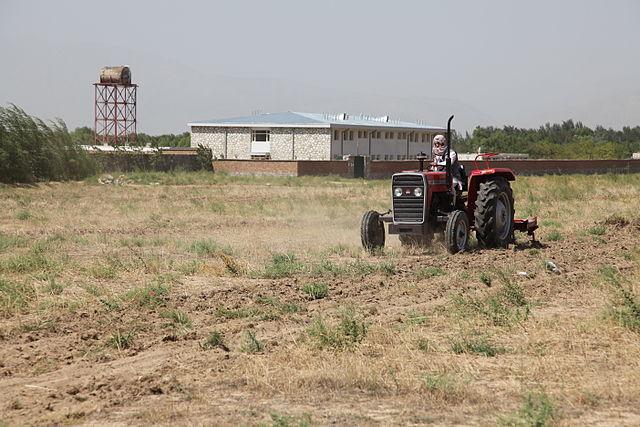
\includegraphics{images/kapisa.jpg}\\
\emph{University Farm: al-Biruni University, Kapisa province,
Afghanistan.}

\hypertarget{example-2}{%
\subsubsection{Example 2}\label{example-2}}

Although it may sound quaint, some variant of the University Farm could
help to physically sustain peeragogues, while putting the project's
{{Heartbeat}} in tune with that of the seasons. In the current
distributed mode, we tend our window boxes and allotment gardens. New
developments should unfold in a \emph{logical order growing out of the
needs of the community} {{[}3{]}}.

\hypertarget{whats-next-in-the-peeragogy-project}{%
\subsubsection{What's Next in the Peeragogy
Project}\label{whats-next-in-the-peeragogy-project}}

\begin{quote}
Actual meeting times to be added
\end{quote}

Identifying and fostering new {{Heartbeats}} and new working groups can
help make the community more robust. This is the time dimension of
spin-off projects described in {{Reduce, reuse, recycle}}.

\hypertarget{references}{%
\subsubsection{References}\label{references}}

\begin{enumerate}
\def\labelenumi{\arabic{enumi}.}
\item
  David M. Dikel, David Kane, and James R. Wilson. 2001. \emph{Software
  architecture: Organizational principles and patterns}. Pearson
  Education.
\item
  Linus Torvalds and Steven Vaughan-Nichols. 2011. Linus Torvalds's
  Lessons on Software Development Management. \emph{Input Output}.
  Retrieved from
  \url{http://web.archive.org/web/20131021211847/http://h30565.www3.hp.com/t5/Feature-Articles/Linus-Torvalds-s-Lessons-on-Software-Development-Management/ba-p/440}
\item
  Booker T Washington. 1901. \emph{Up from slavery}. Doubleday \&
  Company, Inc.
\end{enumerate}

\begin{center}\rule{0.5\linewidth}{0.5pt}\end{center}
